% ============================================================================
% SECTION 1: SYSTEM DESIGN
% ============================================================================
\section{System Design}

\subsection{System Architecture}

HistoryTalk is designed as a modular web platform serving both B2B Educational Institutions (Schools, Classrooms, Teachers, and School Students) and B2C Self-Directed Learners (Customers). The system architecture separates core transactional business operations, user authentication, and institutional lifecycle management from compute-intensive Retrieval-Augmented Generation (RAG), vector similarity search, cross-encoder reranking, and streaming Large Language Model (LLM) roleplay inference.

\begin{figure}[htbp]
    \centering
    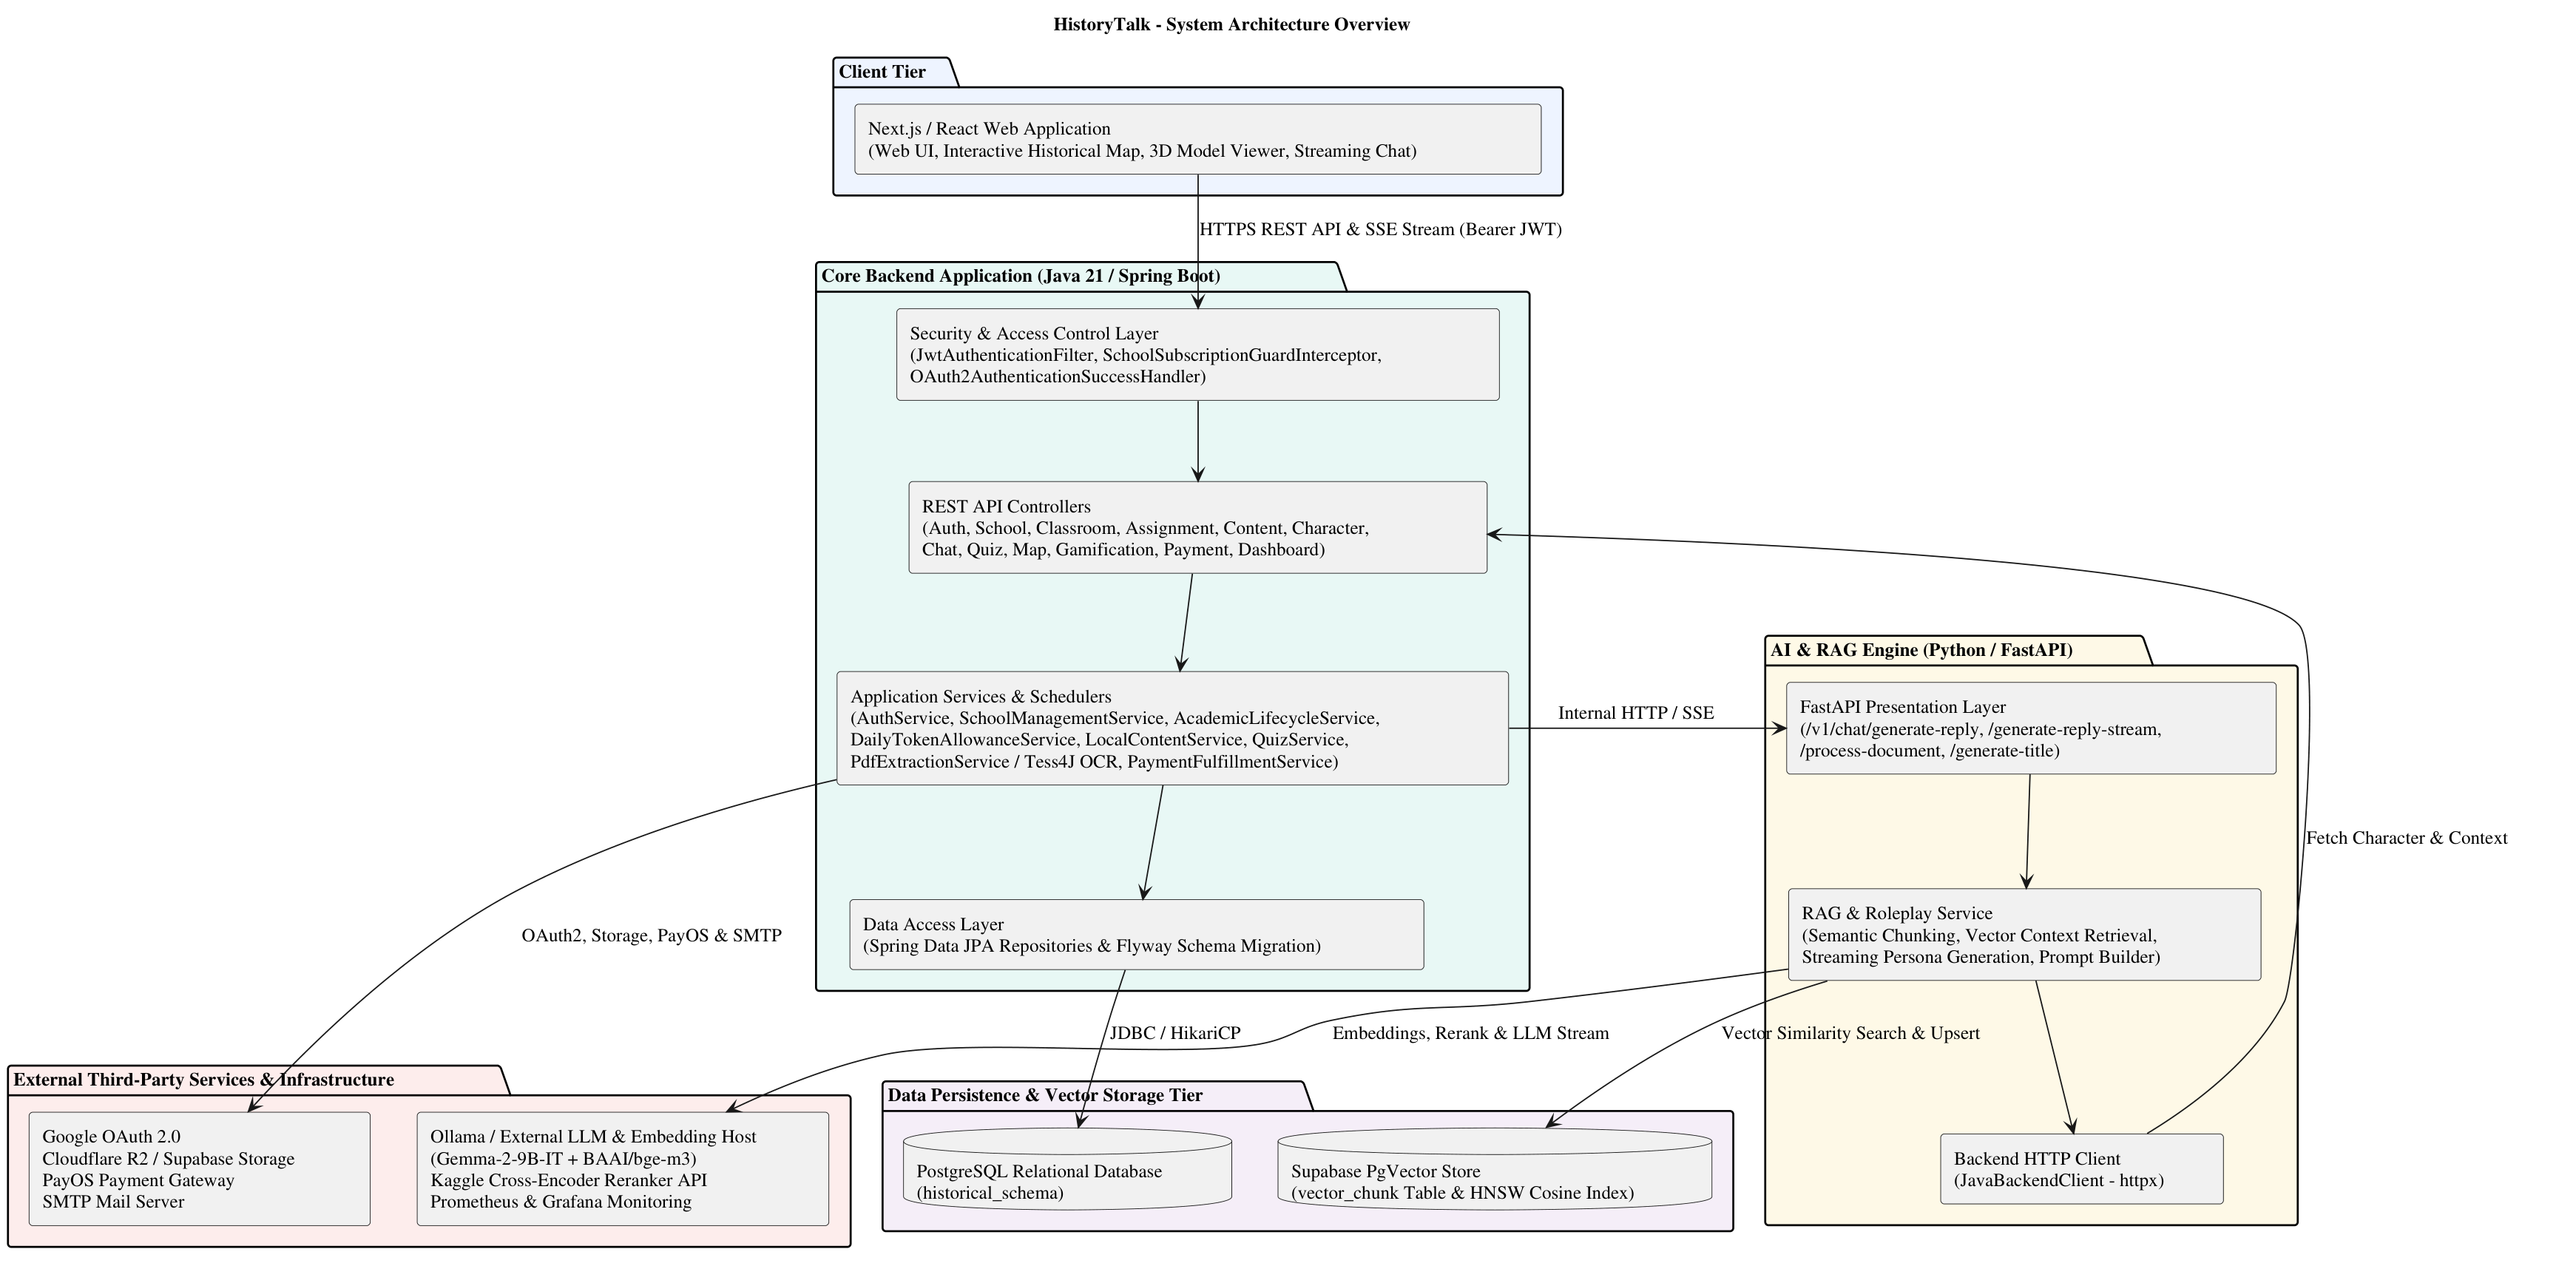
\includegraphics[width=0.92\textwidth,height=0.62\textheight,keepaspectratio]{figures/arch_system_overview.png}
    \caption{HistoryTalk System Architecture Overview}
    \label{fig:arch_system_overview}
\end{figure}

As illustrated in Figure~\ref{fig:arch_system_overview}, the system comprises four primary architectural tiers and external service integrations:

\begin{enumerate}[leftmargin=*]
    \item \textbf{Client Tier:} Provides role-tailored web workspaces for platform actors (Customer, School Student, Teacher, School Admin, Content Admin, and System Admin). It renders interactive spatio-temporal historical battle maps, 3D historical character models, Server-Sent Events (SSE) streaming AI dialogues, timed quizzes, and classroom gradebooks.
    \item \textbf{Core Backend Service:} Acts as the central transactional backend for client traffic. It handles stateless JWT authentication (Jwt\ab Authentication\ab Filter), school academic-year subscription guards (School\ab Subscription\ab Guard\ab Interceptor), multi-tenant data isolation by school\_id, PDF text and OCR extraction (Apache PDFBox and Tess4J), PayOS webhook fulfillment, and Flyway database schema migrations.
    \item \textbf{AI and Hybrid RAG Service:} A dedicated asynchronous Python FastAPI service protected by an internal API key (X-Internal-\ab Api-Key). It executes dynamic semantic chunking, generates 768-dimensional dense embeddings (BAAI/\ab bge-m3), queries Supabase PgVector for context retrieval, invokes the Kaggle Cross-Encoder Reranker, and streams grounded first-person historical persona responses with Socratic reverse-questioning.
    \item \textbf{Data Persistence and Vector Storage Tier:} Combines PostgreSQL (housing relational domain tables in historical\_\ab schema) with Supabase PgVector (storing the vector\_\ab chunk table indexed with HNSW cosine distance for semantic similarity search).
    \item \textbf{External Third-Party Integrations:} Includes Google OAuth 2.0 for Single Sign-On, Cloudflare R2 / Supabase Storage for binary media and 3D models, PayOS Payment Gateway for VietQR checkout and HMAC-SHA256 webhooks, SMTP Mail Server for transactional emails, Ollama / OpenAI-Compatible LLM Host, Kaggle Reranker API, and Prometheus with Grafana for system monitoring.
\end{enumerate}

\newpage
\subsection{Package Diagram}

\subsubsection{Back-end Core Packages}

The Java Core Backend follows a layered and domain-partitioned package organization under com.historytalk, ensuring clean separation between HTTP presentation, security filters, domain business logic, and JPA persistence.

\begin{figure}[htbp]
    \centering
    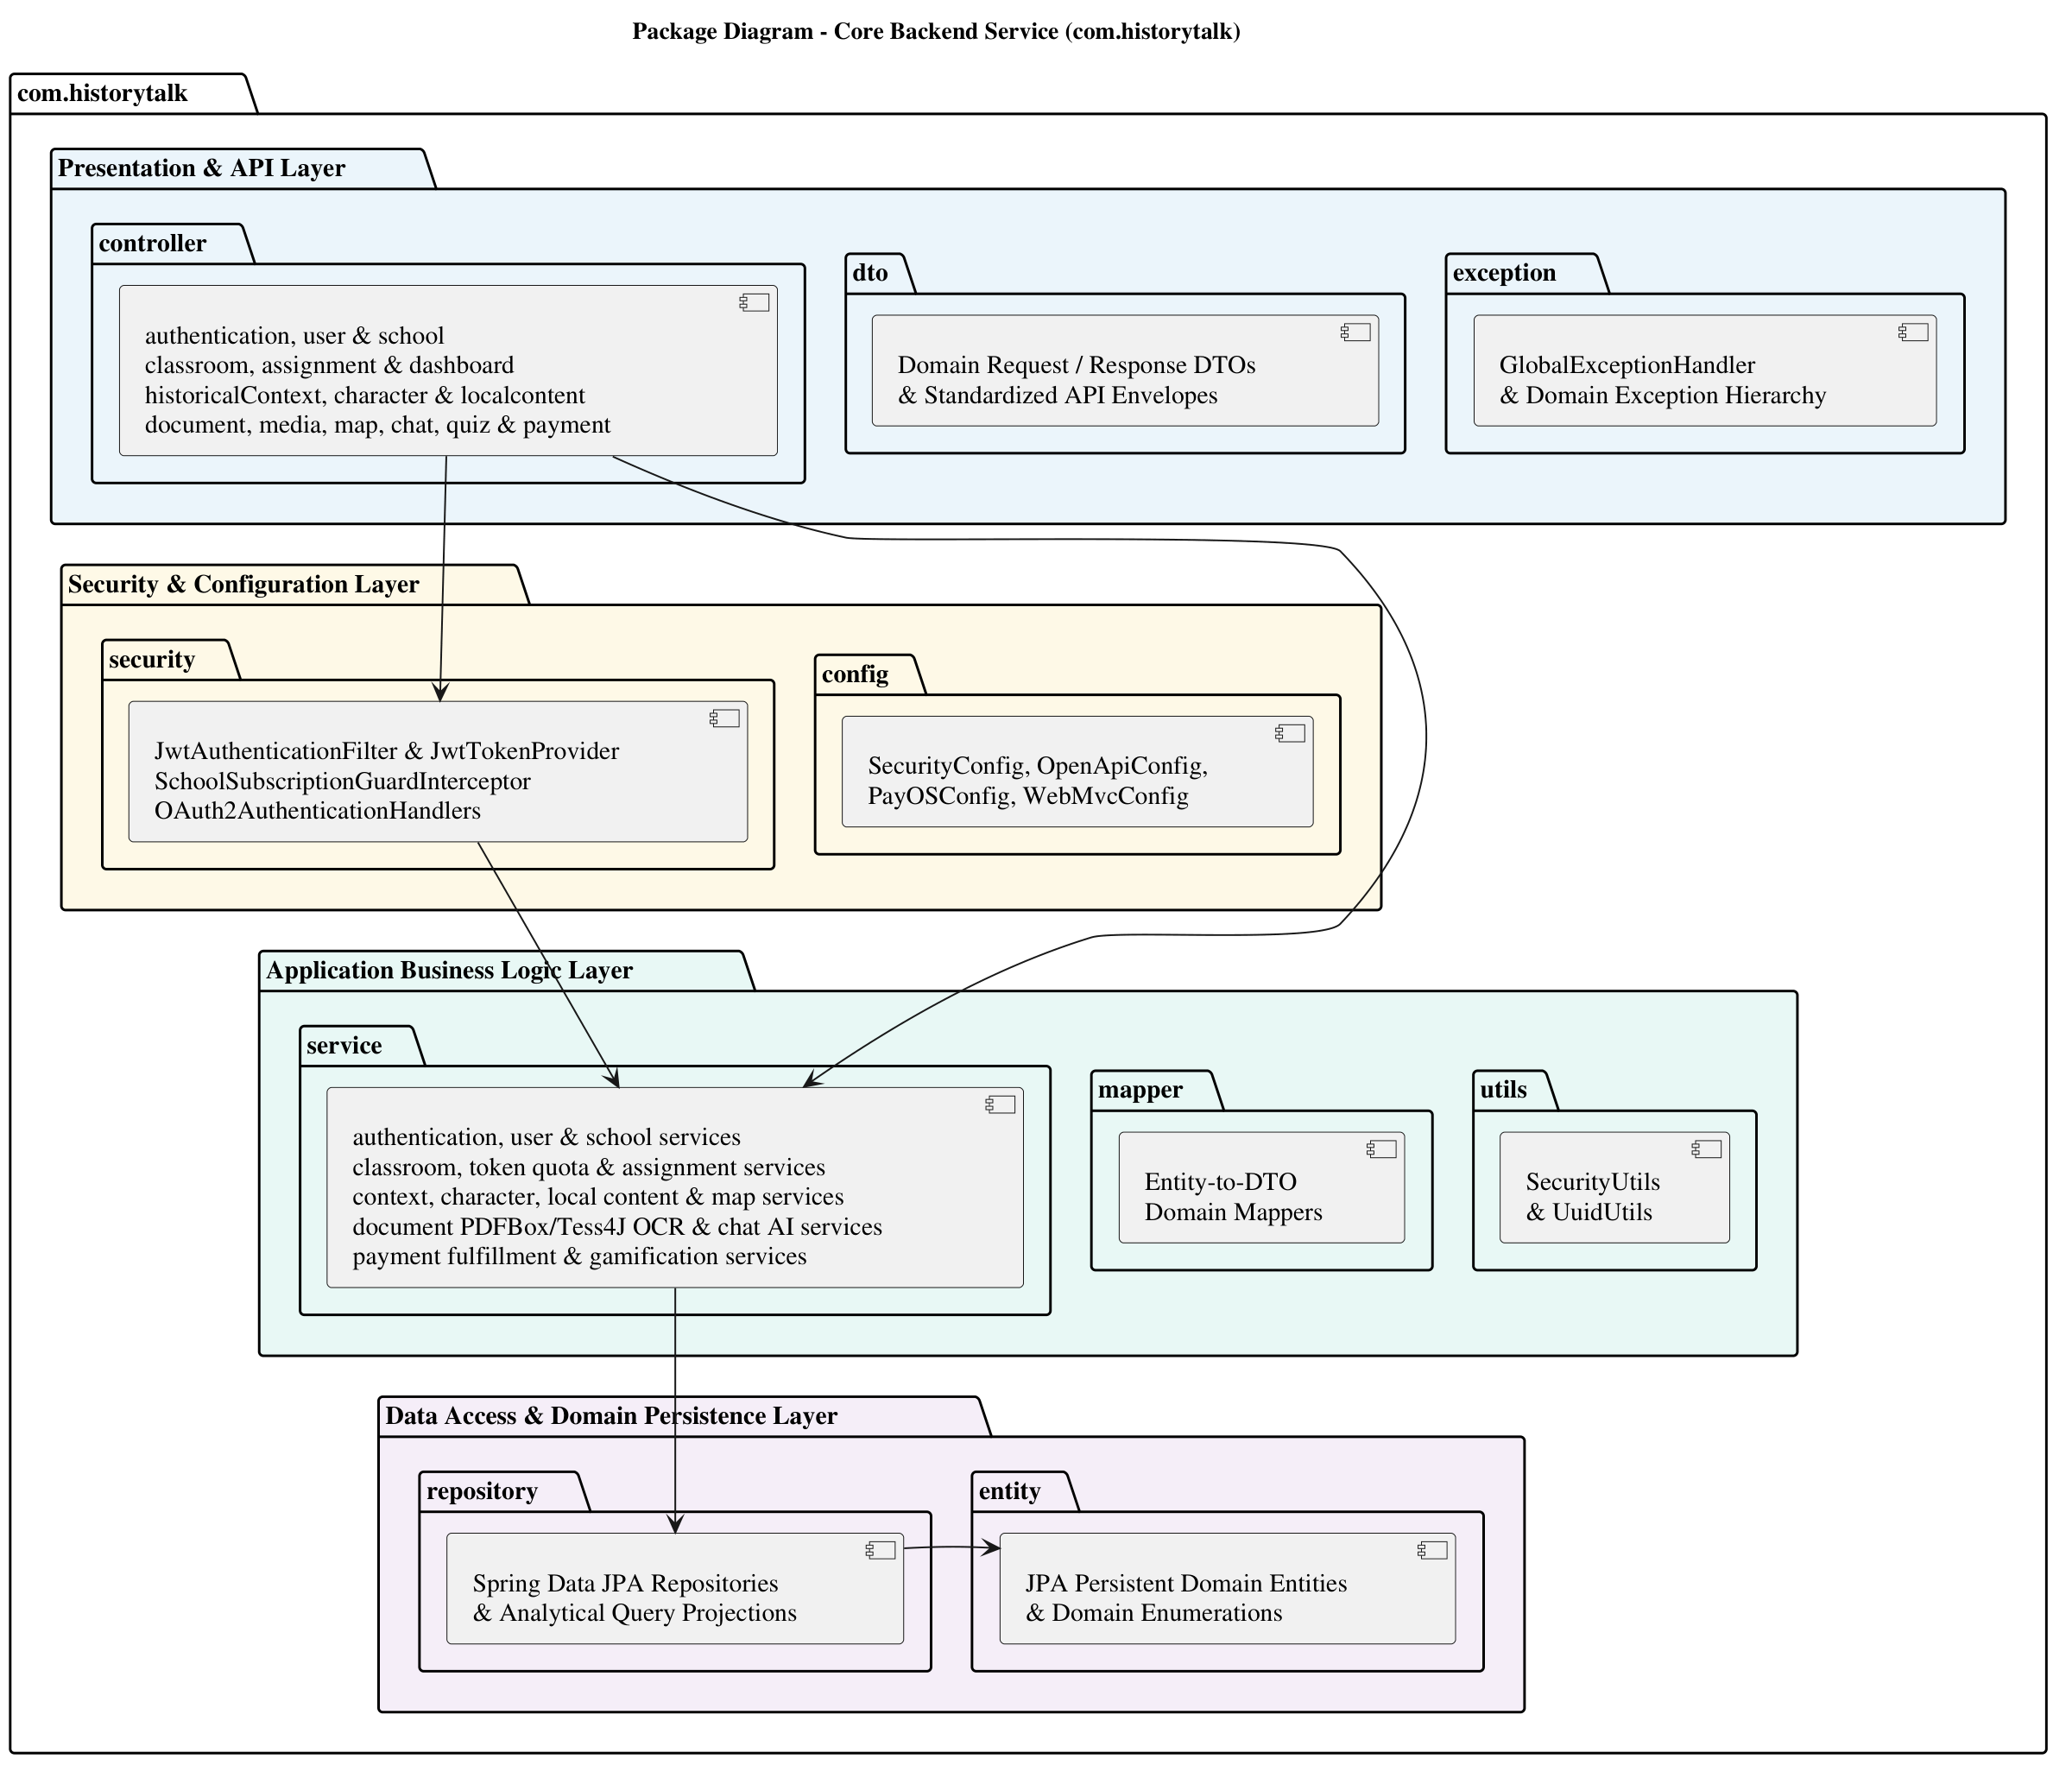
\includegraphics[width=0.88\textwidth,height=0.55\textheight,keepaspectratio]{figures/pkg_backend_java.png}
    \caption{Package Diagram -- Core Backend Service}
    \label{fig:pkg_backend_java}
\end{figure}

\paragraph{Package Descriptions}
\begin{longtable}{|C{0.9cm}|L{4.5cm}|L{8.9cm}|}
\hline
\rowcolor{tableheader}
\textbf{No} & \textbf{Package} & \textbf{Description} \\
\hline
\endhead
01 & com.historytalk.\ab config & Configures Spring Security filter chains (Security\ab Config), OpenAPI/Swagger documentation (OpenApi\ab Config), PayOS SDK client (PayOS\ab Config), OAuth2 properties (OAuth2\ab Properties), and MVC interceptors (School\ab Lifecycle\ab WebMvc\ab Config). \\
\hline
02 & com.historytalk.\ab security & Implements JWT token parsing and signing (JwtToken\ab Provider), request authentication (Jwt\ab Authentication\ab Filter), B2B school subscription enforcement (School\ab Subscription\ab Guard\ab Interceptor), and Google OAuth2 handlers (security.\ab oauth2). \\
\hline
03 & com.historytalk.\ab controller.* & Exposes RESTful API controllers grouped into domain subpackages (authentication, user, school, classroom, assignment, historical\ab Context, character, local\ab content, document, map, chat, quiz, gamification, payment, dashboard, trash). \\
\hline
04 & com.historytalk.\ab dto.* & Encapsulates strongly-typed Request and Response Data Transfer Objects across domain subpackages, along with standardized envelope wrappers (ApiResponse, Paginated\ab ApiResponse, Validation\ab ErrorResponse). \\
\hline
05 & com.historytalk.\ab service.* & Implements and manages core domain business rules, multi-tenant authorization checks, PDF/OCR processing (service.\ab document), CSV bulk student imports (service.\ab school.\ab student), daily token quota and boost workflows (service.\ab school.\ab token), AI service HTTP/SSE communication (service.\ab chat), and resilient PayOS fulfillment (service.\ab payment). \\
\hline
06 & com.historytalk.\ab mapper.* & Maps internal JPA domain entities to external DTO contracts (Character\ab Mapper, User\ab Mapper, Payment\ab Mapper, Tier\ab Mapper) without leaking persistence internals. \\
\hline
07 & com.historytalk.\ab repository.* & Defines Spring Data JPA repository interfaces and analytical query projection interfaces (repository.\ab dashboard) for system, school, and classroom analytics. \\
\hline
08 & com.historytalk.\ab entity.* & Contains persistent JPA domain entities across domain subpackages (user, school, classroom, assignment, historical\ab Context, character, local\ab content, document, map, chat, quiz, gamification, payment) and domain enumerations (entity.\ab enums). \\
\hline
09 & com.historytalk.\ab exception & Centralizes exception handling via Global\ab Exception\ab Handler and domain exception hierarchy (Base\ab Exception, Resource\ab NotFound\ab Exception, Invalid\ab Request\ab Exception, DataConflict\ab Exception, Forbidden\ab Exception, Unauthorized\ab Exception). \\
\hline
10 & com.historytalk.\ab utils & Provides cross-cutting security context helpers (Security\ab Utils) and UUID validation/conversion utilities (Uuid\ab Utils). \\
\hline
\caption{Core Backend Package Descriptions}
\label{tab:pkg_backend_java}
\end{longtable}

\subsubsection{AI and RAG Service Packages}

The Python AI service is organized under src/history\_\ab talk\_ai following a four-layer architecture (presentation, application, dataaccess, and common).

\begin{figure}[htbp]
    \centering
    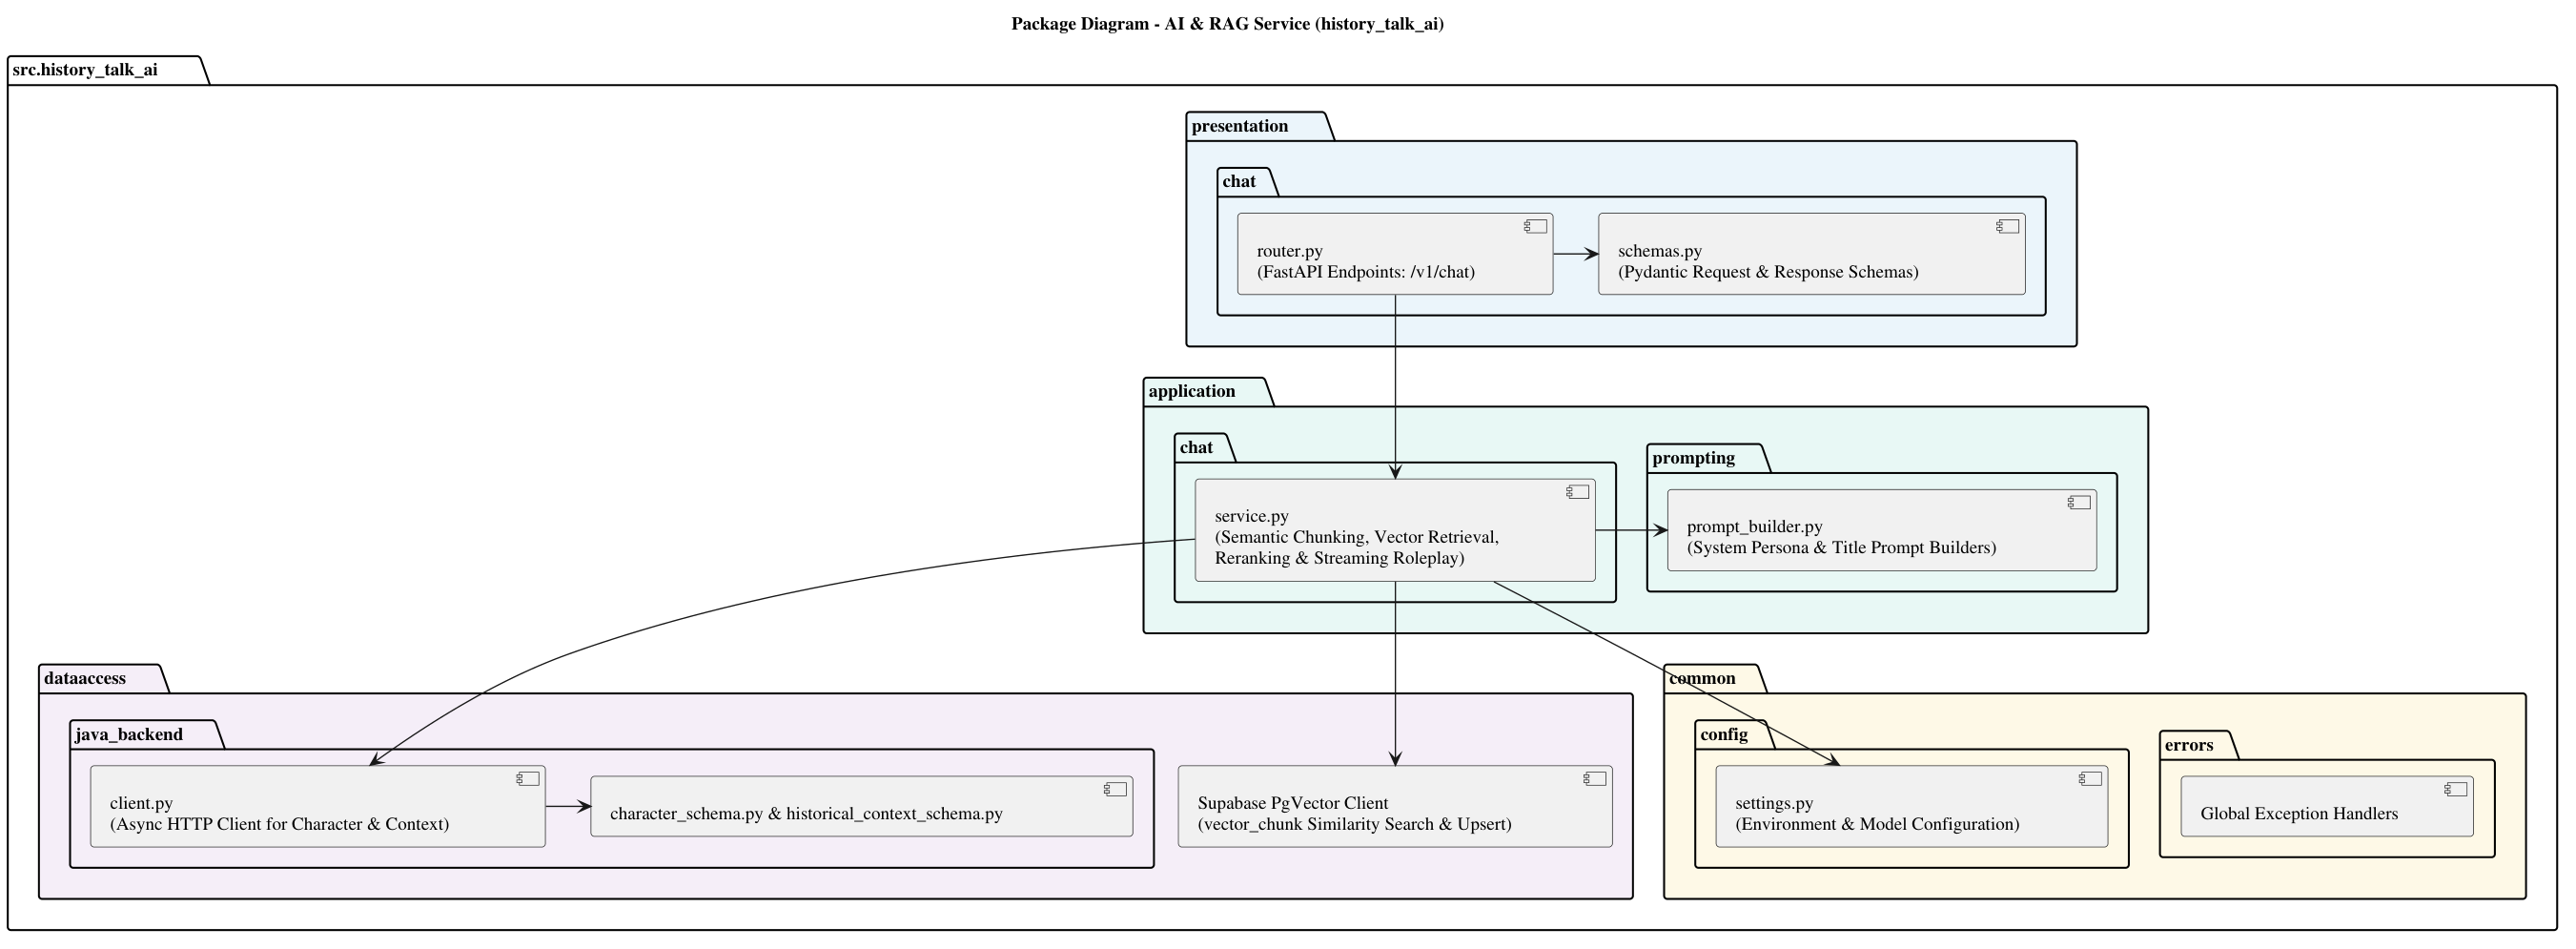
\includegraphics[width=0.85\textwidth,height=0.50\textheight,keepaspectratio]{figures/pkg_backend_ai.png}
    \caption{Package Diagram -- AI and RAG Service}
    \label{fig:pkg_backend_ai}
\end{figure}

\paragraph{Package Descriptions}
\begin{longtable}{|C{0.9cm}|L{4.5cm}|L{8.9cm}|}
\hline
\rowcolor{tableheader}
\textbf{No} & \textbf{Package} & \textbf{Description} \\
\hline
\endhead
01 & presentation.\ab chat.router & Exposes FastAPI endpoints under /v1/chat (/generate-\ab reply, /generate-\ab reply-stream, /generate-\ab title, /process-\ab document, and DELETE /documents/\ab \{doc\_id\}) secured by internal API key validation. \\
\hline
02 & presentation.\ab chat.schemas & Defines Pydantic request and response models (Generate\ab ReplyRequest, Generate\ab ReplyResponse, Message\ab HistoryItem, Process\ab Document\ab Request, Generate\ab TitleRequest). \\
\hline
03 & application.\ab chat.service & Implements the core RAG and LLM pipeline: dynamic semantic chunking (\_semantic\_\ab chunking), BGE-M3 embedding generation (get\_\ab embedding\_\ab from\_ollama), Supabase vector similarity retrieval and Kaggle reranking (retrieve\_\ab history\_\ab context), and SSE streaming roleplay (generate\_\ab reply\_\ab stream). \\
\hline
04 & application.\ab prompting & Houses prompt\_\ab builder.py (build\_chat\_\ab system\_prompt, build\_title\_\ab system\_prompt), constructing first-person historical persona instructions, anti-hallucination constraints, and Socratic questioning rules. \\
\hline
05 & dataaccess.\ab java\_backend & Implements asynchronous httpx client (client.py) and typed domain schemas (character\_\ab schema.py, historical\_\ab context\_\ab schema.py) to fetch character biographies, eras, and context metadata from the Java Core Backend. \\
\hline
06 & common.config & Manages environment configuration via pydantic-\ab settings (settings.py), binding LLM provider routing (ollama vs. external), model parameters, Supabase credentials, and timeouts. \\
\hline
07 & common.errors & Provides global FastAPI exception handlers and structured JSON error responses for upstream timeout, embedding, or LLM inference failures. \\
\hline
\caption{AI and RAG Service Package Descriptions}
\label{tab:pkg_backend_ai}
\end{longtable}

\subsubsection{Front-end Web Application Packages}

\begin{figure}[htbp]
    \centering
    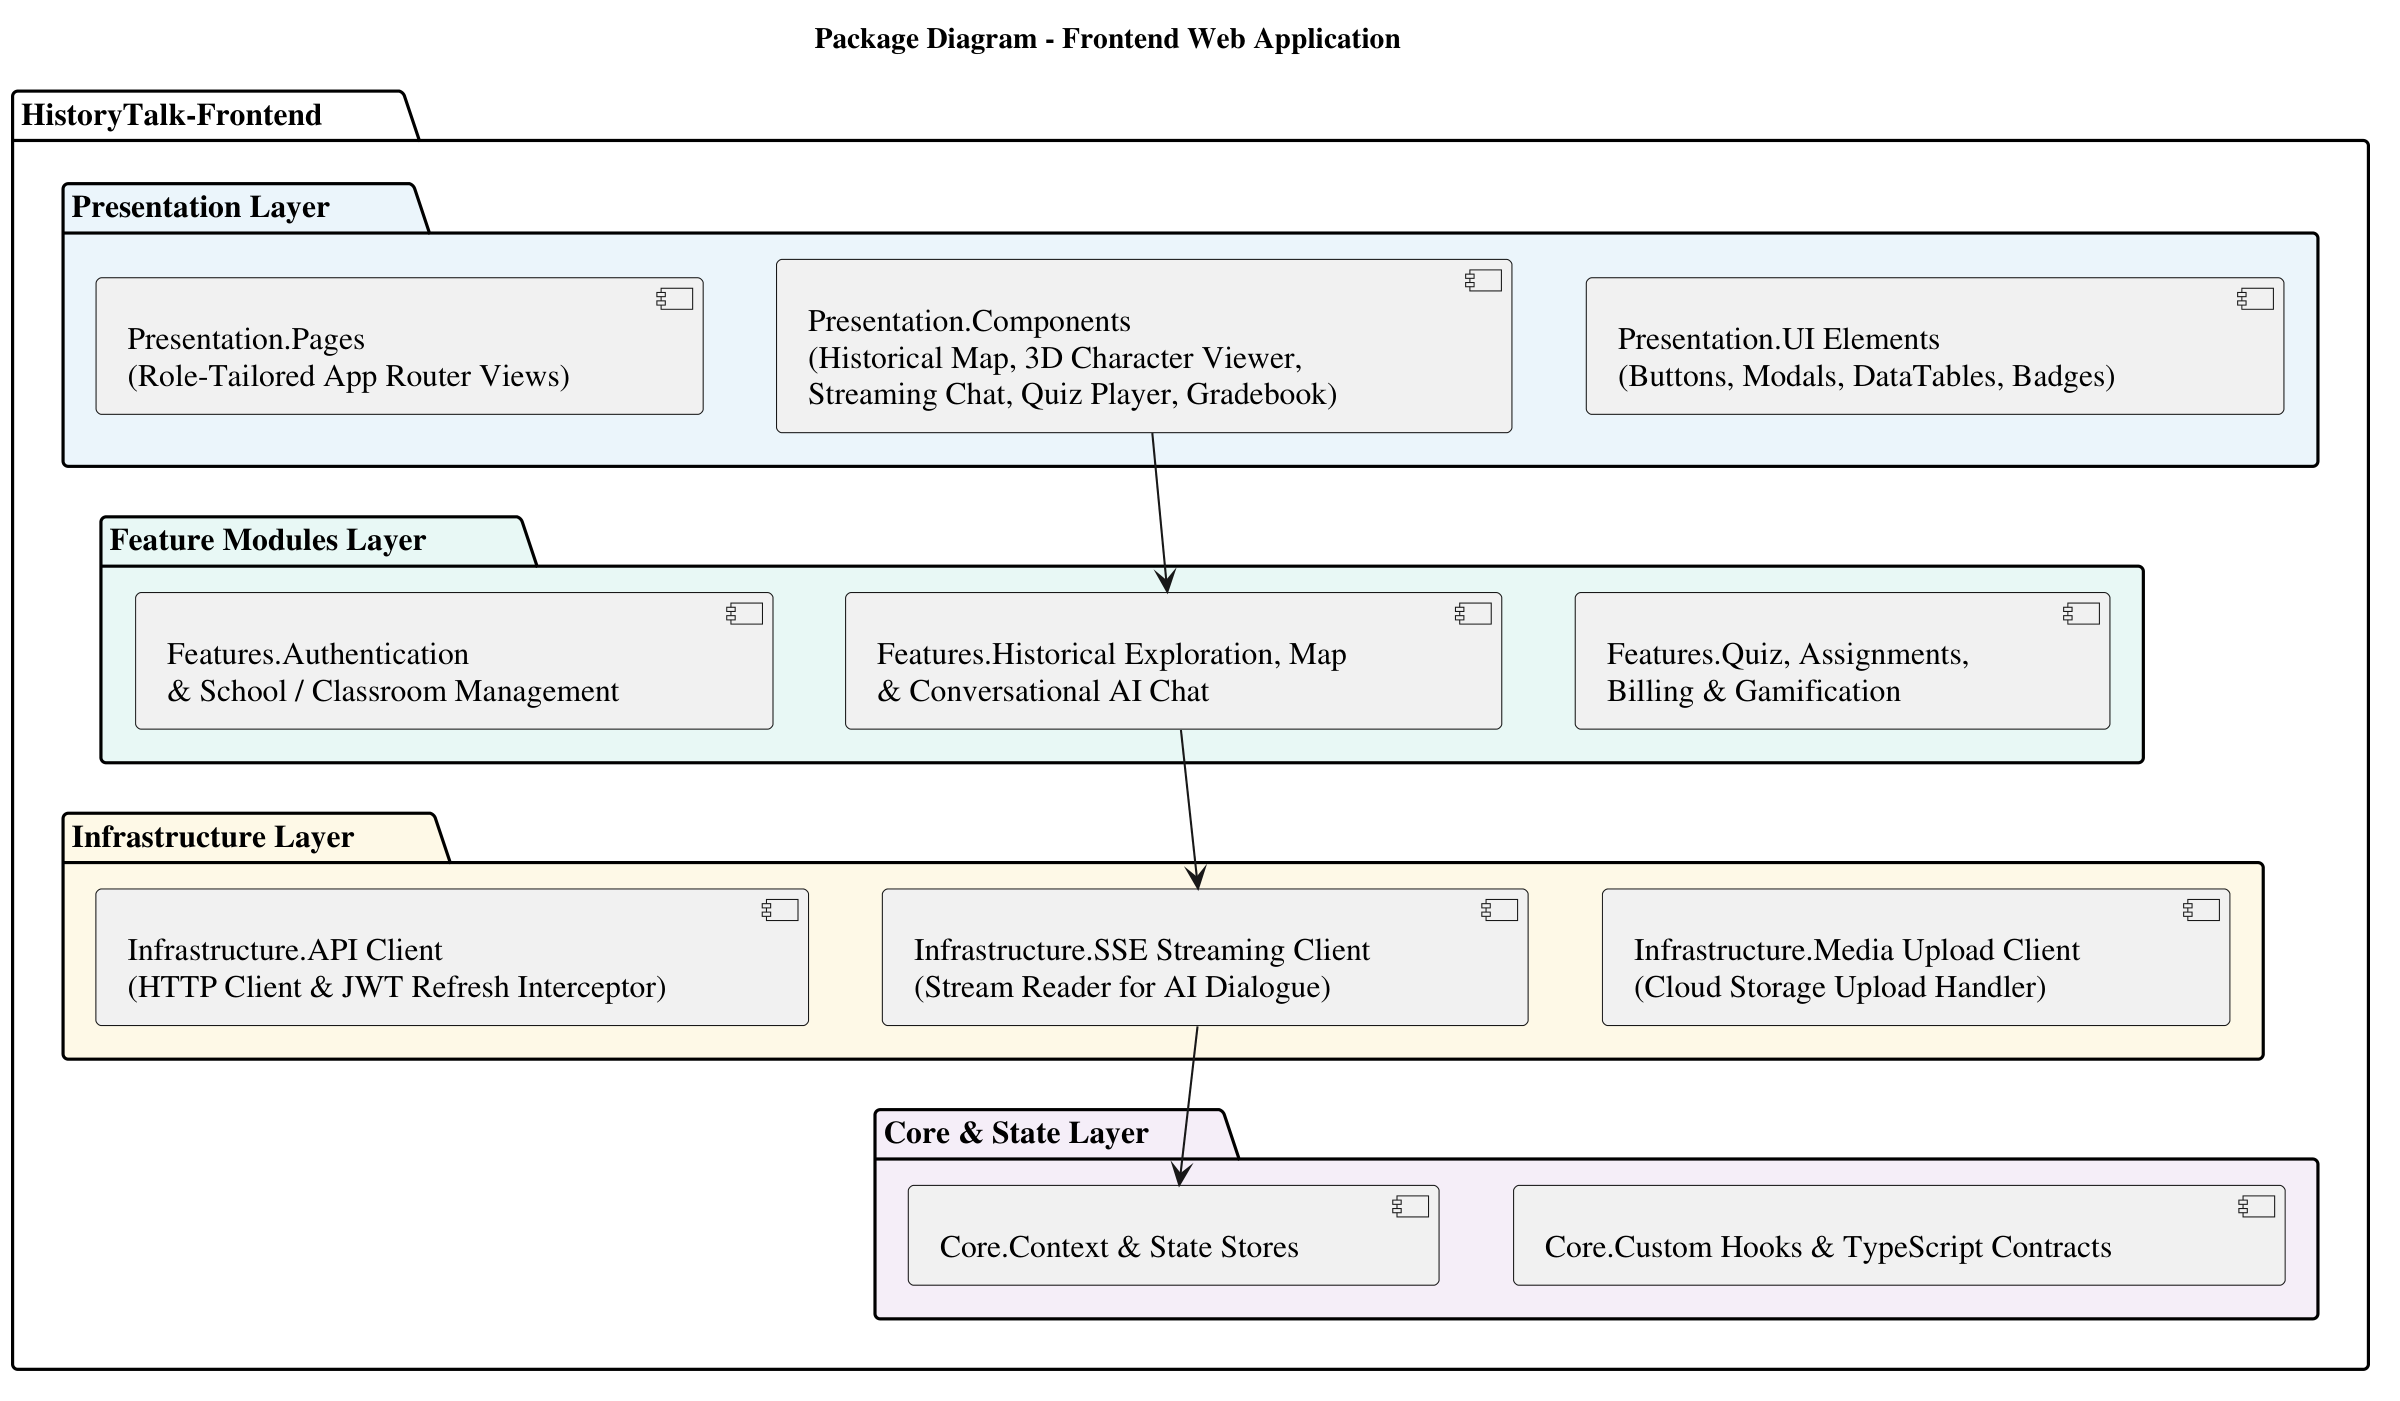
\includegraphics[width=0.88\textwidth,height=0.52\textheight,keepaspectratio]{figures/pkg_frontend_web.png}
    \caption{Package Diagram -- Frontend Web Application}
    \label{fig:pkg_frontend_web}
\end{figure}

\paragraph{Package Descriptions}
\begin{longtable}{|C{0.9cm}|L{4.5cm}|L{8.9cm}|}
\hline
\rowcolor{tableheader}
\textbf{No} & \textbf{Package} & \textbf{Description} \\
\hline
\endhead
01 & Presentation.\ab Pages & Next.js App Router views segregated by actor role: Public/Customer Portal, School Student Learning Workspace, Teacher Classroom Console, School Admin Portal, Content Admin Studio, and System Admin Dashboard. \\
\hline
02 & Presentation.\ab Components & Reusable domain widgets including BattleMap\ab Canvas (interactive map pins and animated route arrows), Character3D\ab Viewer (3D model viewer), Streaming\ab ChatBox, QuizPlayer, and Gradebook\ab Table. \\
\hline
03 & Presentation.\ab UI Elements & Atomic design primitives (Buttons, Dialog Modals, DataTables, Pagination, StatusBadges, Toast notifications, and Skeletons). \\
\hline
04 & Features.\ab Authentication & Handles credential login, Google OAuth2 callback processing, mandatory first-login password change for imported school students, and role-based route protection. \\
\hline
05 & Features.\ab School \& Classroom & Manages B2B school onboarding, academic year lifecycle rollover, classroom creation, CSV student roster bulk import, and daily token quota/boost review workflows. \\
\hline
06 & Features.\ab Historical Exploration \& Map & Drives timeline browsing by EventEra and Event\ab Category, interactive battle-map overlays, camera viewpoint focuses (MapFocus), and school-owned local history content workflows. \\
\hline
07 & Features.\ab Conversational AI Chat & Manages character roleplay sessions, real-time SSE token streaming, clickable suggested follow-up questions, and cited historical quotes display. \\
\hline
08 & Features.\ab Quiz \& Assignments & Implements interactive quiz players (MULTIPLE\_\ab CHOICE, FILL\_IN\_\ab BLANK, MATCHING), question bank CSV import, teacher assignment dispatch, and automated submission tracking. \\
\hline
09 & Features.\ab Billing \& Gamification & Manages B2C tier upgrades via PayOS QR checkout, order status polling, daily streak check-ins, and daily quest token rewards. \\
\hline
10 & Infrastructure & Configures HTTP client interceptors with automatic JWT refresh token rotation, SSE stream readers, and direct binary media uploads to cloud storage. \\
\hline
11 & Core / State & Provides React contexts, state stores, custom hooks (useAuth, useStreaming\ab Chat, useToken\ab Balance), and TypeScript DTO interfaces synchronized with backend API specs. \\
\hline
\caption{Frontend Web Application Package Descriptions}
\label{tab:pkg_frontend_web}
\end{longtable}
